\chapter{最小割数量的敏感度分析}
\section{最小割数量的敏感度}
在求解近似最小割的过程中,需要尽可能找到多的解,
然而差分隐私的算法要求一条边的存在与否对输出的影响不能过大。
因此,需要首先对最小割数量进行敏感性进行定量分析,
才能设计出恰当的噪声添加值。

假设现在有两个边相邻的图$G,G'$,其中$G'$由在$G$中加入一条边权为$1$的边$(u,v)$得到。
不妨假设最小割数量计算函数的输入与输出都以适当的二进制形式进行编码,
可以得到最小割数量的敏感度为$d=|M_G-M_{G'}|$。

我们知道,对于任意图$G$,最小割数量满足$1\leq M_G\leq n^2$,因此$0\leq d\leq n^2$。


\begin{lemma}
  \label{lemma:mingganN}
  对于任意$n\geq 3$,存在图$G,G'$的构造方法,使得最小割数量的敏感度为$\Omega(n^2)$。
\end{lemma}
\begin{proof}
  我们不妨将点集中的点编号,用$v_1$至$v_n$表示。下面给出构造方法:
  图$G$由如下方法生成,连接$v_1$与$v_2$,$v_2$与$v_n$,并对于所有整数$2\leq i<n$,连接$v_i$和$v_{i+1}$;
  图$G'$由图$G$的基础上,增加一条连接$v_1$和$v_2$的边得到。
  
  这里的连边均为$1$,因此图$G$的最小割值为$1$,唯一的方案是$(\{v_1\},V\backslash v_1)$,因此$M_G=1$。
  图$G'$的最小割值为$2$,此时对于任意$2\leq i\leq j\leq n$,
  $(\{v_i,\ldots,v_j\},V\backslash \{v_i,\ldots,v_j\})$都是一个最小割,
  因此$M_{G'}=\frac{n^2-n}2$。在这种构造方法下,$d=\Omega(n^2)$。
\end{proof}
\begin{figure}[htb]
    \centering
    \subfloat[图$G$]{
      \label{1}
      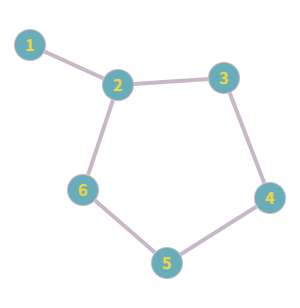
\includegraphics[height=5cm]{figures/graph001.png}}\hspace{4em}
    \subfloat[图$G'$]{
      \label{2}
      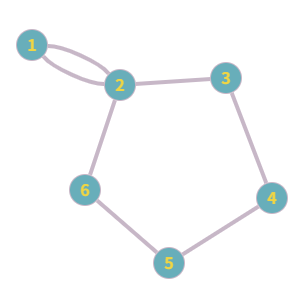
\includegraphics[height=5cm]{figures/graph002.png}}
    \caption{$n=6$时的构造示例}
    \label{fig:exA}
\end{figure}
图\ref{fig:exA}给出了一种$n=6$时的构造示例。
引理表明,边相邻图的最小割数量的敏感度在一些情况下特别高,
高敏感度意味着需要添加较大噪声,进而使得差分隐私下发布的最小割数量可用性较低。
因此在设计算法时,需要引入一些额外的约束条件。
\section{约束条件下的敏感度}
给定图$G$,在加入一条单位边后,最小割的割值可能增加,也可能保持不变。
引理\ref{lemma:mingganN}指出,若图有一个割值为$x$的割和较多割值为$x+1$的割,
那么加边导致最小割的割值提高$1$后,会使最小割的数量出现较大的增幅。
因此,为了得到可用的结果,可以加入边相邻图的最小割值相同这一额外限制条件,
也就是说,图$G,G'$满足$\Phi_G=\Phi_{G'}$。在本章的后文中,如未特殊说明,图$G,G'$将默认满足这一性质。


标准仙人掌图表示法包含了图所有最小割的信息,因此其结构参数有助于对问题分析的精细性。所以,
对于一个图$G$以及其标准仙人掌图表示法$(\Gamma,\varphi)$,我们引入以下参数来描述图的结构:
\begin{itemize}
  % \item $\alpha_{n}$:图$G$的点数,即$|V_G|$%平均用的吧
  \item $\alpha_{g}$:标准仙人掌图表示法的点数,即$|V_{\Gamma}|$。
  \item $\alpha_{p}$:标准仙人掌图表示中所有点$v$对应的$|\varphi^{-1}(v)|$的最大值%平均用的吧
  \item $\alpha_{c}$:标准仙人掌图表示中环的数量。
  \item $\alpha_{r}$:标准仙人掌图表示中环长度的最大值。
  \item $\alpha_{d}$:标准仙人掌图表示中树结构的直径,也就是所有图上简单路径中,非环边数量的最大值。
  % \item $\beta_{p}$:图$G$的$p$割数量。
  % \item $\beta_{t}$:图$G$的$t$割数量。
\end{itemize}


在$G$中加入一条边权为$1$的边$(u,v)$得到$G'$,
接下来我们分析这条边$(u,v)$在标准仙人掌图表示法$(\Gamma,\varphi)$中的位置与最小割数量变化量的关系。
首先,若$\varphi(u)=\varphi(v)$,那么说明$u,v$之间不被任何最小割分隔开,
在仙人掌图表示法中它们已经被视为连通性很高的两个点,因此加入边$(u,v)$对最小割数量没有任何影响。

若$\varphi(u)\neq\varphi(v)$,我们不妨令$U=\varphi(u)$,$V=\varphi(V)$。
根据标准仙人掌图表示法的构造过程可知,其表示最小割的结构主要有树表示和每个$p$束对应的结构环两部分。
树表示中$U$到$V$路径上的所有$p$割都将不再是最小割,路径上所有$p$束对应的结构环代表的$t$割都会变少。
具体来说,对于一个$p$束$S$的结构环$G_S$,令$U\in x_{R'},V\in x_{R''}$,
所有将$x_{R'}$与$x_{R''}$分开的$t$割都将不再是最小割。

接下来对环上的情况进行定量分析。令$f(x)$为长度为$x$的环表示的$t$割数量,则
\begin{equation*}
  f(x)=\begin{cases}
    \frac{x(x-3)}2&x\geq 3\\0&1\leq x\leq 2\end{cases}  
\end{equation*}
假设结构环$G_S$的环长为$l$,$x_{R'}$与$x_{R''}$在环上的距离为$t$(满足$t\leq l-t$),
那么最小割的减少量为
\begin{equation*}
  g(l,t)=f(l)-f(t)-f(l-t)-[t\geq 3]-[l-t\geq 3]
\end{equation*}
令$G(l)=\max_{t=1}^{l-1}g(l,t)$,我们不妨对$l,t$的值进行讨论来得到该函数的取值:
当$1\leq l\leq 3$时,环上不包含$t$割,因此$G(l)=0$;
当$l=4$时,取$t=2$为极值,$G(4)=2$;
当$l\geq 5$时,由于$l-t\geq t$,且$f$为单调函数
因此我们只需要讨论$t=2,t\geq 3$这两种情况。
\begin{itemize}
  \item 当$t=2$时,$g(l,2)=f(l)-f(l-2)-1=2l-6$;
  \item 当$t\geq 3$时,$g(l,t)=f(l)-f(t)-f(l-t)-2=-(t-\frac l2)^2+\frac{l^2}4-2$。
\end{itemize}
当$l=5$时,$t\leq 2$,因此$G(5)=g(5,2)=4$。
当$l\geq 6$时,$g(l,t)$的极小值在$t=\left\lfloor\frac l2\right\rfloor$时取到,
此时$g(l,t)\geq g(l,2)$。综上,可以得到
\begin{equation*}
  G(l)=\max{\{0,\lfloor\frac{l^2}4-2\rfloor\}}
\end{equation*}

除此之外,可以发现,加入$(u,v)$使最小割的割值增加一的情况只有在$\varphi(u)\neq\varphi(v)$,
标准仙人掌图表示法中的树表示是一条链,且$\varphi(u),\varphi(v)$分别是链的两个端点时出现。

接下来,我们给出最小割数量变化范围的表达式。

\begin{theorem}
    给定边相邻图$G,G'$,其中$G'$由在$G$中加入一条边权为$1$的边$(u,v)$得到。那么有
    \begin{equation*}
      M_G-\min{\{\alpha_d,\alpha_c,\frac{\alpha_g}{\alpha_r}\}}·\max{\{0,\lfloor\frac{\alpha_r^2}4-2\rfloor\}}-\alpha_d \leq M_{G'}\leq M_G
    \end{equation*}

\end{theorem}

最小割数量的变化还可以由$M_G$本身的值进行估计。
对于一个长度$l\geq 4$的环$G_S$,其表示的$t$割有$f(l)=\frac{l(l-3)}2$个,
边$(u,v)$经过它是会使其最小割数量减少至多$G(l)= \lfloor\frac{l^2}4-2\rfloor$。
此外不难证明,该$p$束$S$连接的不涉及$x_{R'},x_{R''}$的至少$l-2$条边对应的$p$割在加边后仍然为最小割。
因此,与该$p$束$S$相关的最小割的数量为$\frac{l^2-l-4}2$,减少量至多为$\lfloor\frac{l^2}4-2\rfloor$。
\begin{theorem}
  对于任意加边$(u,v)$,存在一种最小割分配方案,满足每个最小割至多分配至一个$p$束中,使得
  每个$p$束$S$损失的最小割数量不超过其分配量与$|G_S|$和的一半。
\end{theorem}

\begin{proof}
  按上文方法分配最小割后,$p$束$S$分配到的最小割数量为$\frac{l^2-l-4}2$,$G_S=l$
  其损失的最小割数量为$\lfloor\frac{l^2}4-2\rfloor$。有
  \begin{equation*}
    \frac{l^2-l-4}2+l=\frac{l^2+l-4}2\geq \frac{l^2}2-4\geq 2\lfloor\frac{l^2}4-2\rfloor
  \end{equation*}
\end{proof}
因此我们可以给出基于$M_G$的估计。

% 我们再给出最小割数量的估计
% \begin{theorem}
%   给定图$G$,有
%   \begin{equation*}
%     \max{\{0,\frac{\alpha_r(\alpha_r-3)}2\}}+\alpha_d\leq M_G\leq \min{\{\alpha_c,\frac{\alpha_g}{\alpha_r}\}}·\max{\{0,\frac{\alpha_r(\alpha_r-3)}2\}}+\alpha_d
%   \end{equation*}

% \end{theorem}
\begin{theorem}
  \label{sen}
  给定边相邻图$G,G'$,其中$G'$由在$G$中加入一条边权为$1$的边$(u,v)$得到。那么有
  \begin{equation*}
    \frac{M_G}2-1.5n \leq M_{G'}\leq M_G
  \end{equation*}

\end{theorem}
该定理给出了最小割数量敏感度的上界$\frac{M_G}2+1.5n$。
接下来将给出一个构造来说明这个上界可以近似的达到,
该构造下的最小割数量的敏感度与定理中最坏情况下的敏感度仅相差一个常乘法系数,
图$G$构造方法如下:
将$(1-\alpha) n$的点用边权$c$连成一条链,设链的两端分别为$v_1,v_2$;
将$\alpha n\geq 4$的点用边权$\frac c2$连成一个环,设环的一个对角线连接的两个点为$v_3,v_4$;
最后将$v_2,v_3$用边权为$c$的边相连,完成构造。

首先,$M_G=n+\frac{\alpha n(\alpha n-3)}2$。敏感度最高的加边是$(v_1,v_4)$,
敏感度$M_G-M_{G'}=\lfloor\frac{\alpha^2 n^2}4\rfloor+(1-\alpha) n$。
不失一般性地取$\alpha=\frac 12$,可得$M_G=\frac{n(n+2)}8$,$M_G-M_{G'}=\lfloor\frac{n^2}{16}\rfloor+\frac 12n$。
此时有
\begin{equation*}
  \frac{M_G}2+\frac32n= \frac{n^2}{16}+\frac{13}{8}n\leq 4(M_G-M_{G'})
\end{equation*}


\section{平均敏感度}
前面的分析表明,在最坏情况下,最小割数量的敏感度较高。这一小节将通过平均敏感度分析造成高敏感度的情况的频次。

在平均敏感性的通常定义中,其边相邻的图以删边的形式给出。\cite{varma2023average}
然而在前文描述边相邻图时,由于删边会较大的改变仙人掌表示的结构,因此用加边的形式描述了$G,G'$间的关系。
这一部分将沿用加边的方法来定义平均敏感度。
通过删边形式的平均敏感度,可以估计一个图算法在规模较大的子图上的输出和完整图上的输出差异,
改为加边形式会弱化这一功能。加边形式的平均敏感度能对应前文的分析,并给出最小割数量变化值的期望。

\begin{definition}
  图算法$A$的平均敏感度为
  \begin{equation*}
    \mathbb E_{e\in V^2,\Phi(G)=\Phi((V,E\cup\{e\}))}[d_{Ham}(A(G),A((V,E\cup\{e\})))]
  \end{equation*}
\end{definition}

考虑这样一种$G$的构造,生成一个规模为$\frac 13n$的图$G_t$,
使得$G_t$在加入边$(u,v)$时得到该规模下最高的敏感度$W(\frac 13n)$,
接下来将$\frac 13n$个点与$u$用极大的边权相连,将$\frac 13n$个点与$v$用极大的边权相连。
此时最小割数量函数$M$的平均敏感度满足
\begin{equation*}
  \mathbb E_{e\in V^2,\Phi(G)=\Phi(G+e)}[d_{Ham}(M(G),M(G+e))]\geq \frac{\frac 13n(\frac 13n-1)}{n(n-1)}W(\frac 13n)
\end{equation*}
最高敏感度$W$是一个$n$的不超过二次的一个多项式。综上,存在一个常数$\beta$使得在该构造下
\begin{equation*}
  \mathbb E_{e\in V^2,\Phi(G)=\Phi(G+e)}[d_{Ham}(M(G),M(G+e))]\geq \beta W(n)
\end{equation*}
分析表明,在最坏情况下,导致高敏感度的加边出现频率的期望较高。